\section{Continuous functions}

A function \(f\) maps elements of a set \(A\) to elements of another set \(B\). We denote this as \(f : A \rightarrow B\). In practice, most functions we consider will have type \(\mathbb{R} \rightarrow \mathbb{R}\).

If a function maps a number of \(x\) to its square \(x^2\), we can denote this by \(x \mapsto x^2\). (Note the difference in the arrow symbol used --- the symbol \(\mapsto\) is read as ``maps to''.)

A function \(y = f(x)\) can be represented graphically as the set of points \((x, y)\). See figure \ref{fig:Ch02-quadratic-graph}.

\begin{figure}[H]
    \centering

    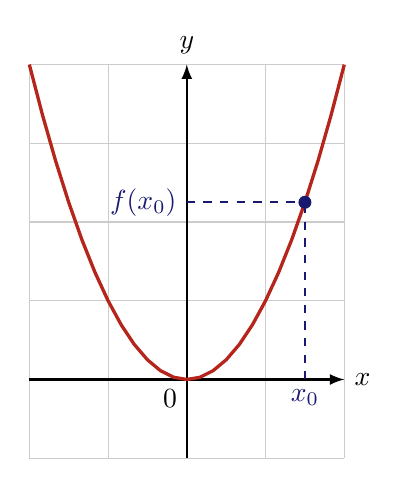
\begin{tikzpicture}
        \draw[thin,gray!40] (-2,-1) grid (2, 4);
        \draw[thick, ->, >=latex] (-2,0)--(2,0) node[right]{\(x\)};
        \draw[thick, ->, >=latex] (0,-1)--(0,4) node[above]{\(y\)};
        \draw (0, 0) node[below left] {0};

        \draw [BrickRed, very thick, domain=-2:2] plot (\x, {\x*\x}); 

        \draw[MidnightBlue, dashed, thick] (1.5, 0) node[below]{\(x_0\)} --(1.5, 2.25);
        \draw[MidnightBlue, dashed, thick] (0, 2.25) node[left]{\(f(x_0)\)} --(1.5, 2.25);

        \filldraw[radius=0.075, MidnightBlue] (1.5,2.25) circle;
    \end{tikzpicture}
    
    \caption{The graph of the function \(y = x^2\).}
    \label{fig:Ch02-quadratic-graph}
\end{figure}

In the next few subsections, we will be looking at some classic mathematical functions.


\subsection{Trigonometric functions}

Consider a point \(P\) on the unit circle. If we let \(\theta\) be the angle between \(OP\) and the horizontal axis, then the coordinates of \(P\) can be expressed as \((\cos{\theta},\; \sin{\theta})\). This is illustrated in figure \ref{fig:Ch02-trig-funcs-on-unit-circle}.

\begin{figure}[H]
    \centering

    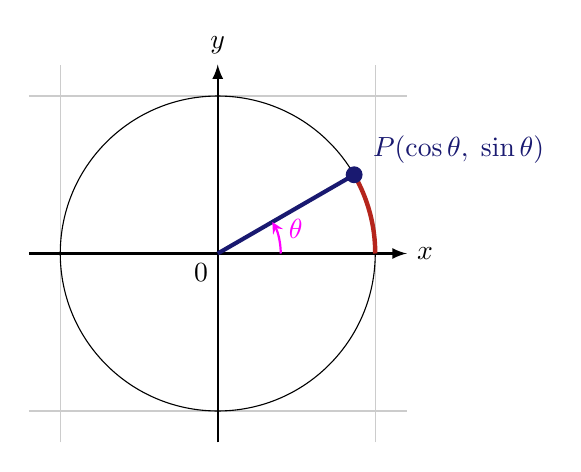
\begin{tikzpicture}[scale=2]
        \draw[thin,gray!40] (-1.2,-1.2) grid (1.2, 1.2);

        \draw[radius=1] (0, 0) circle;

        \draw[thick, ->, >=latex] (-1.2,0)--(1.2,0) node[right]{\(x\)};
        \draw[thick, ->, >=latex] (0,-1.2)--(0,1.2) node[above]{\(y\)};
        \draw (0, 0) node[below left] {\(0\)};

        \draw[BrickRed, ultra thick] (1, 0) arc (0:30:1);

        \filldraw[radius=0.05, MidnightBlue] ({sqrt(3)/2}, 0.5) circle;
        \draw[line width=1.5pt, MidnightBlue] (0,0)--({sqrt(3)/2}, 0.5) node[anchor=south west]{\(\;P(\cos{\theta},\; \sin{\theta})\)};
        \draw[-stealth,Fuchsia, thick] (0.4, 0) arc (0:30:0.4) node[pos=0.5, anchor=west, shift={(0, 0.1)}]{\(\theta\)};

        
    \end{tikzpicture}
    
    \caption{The trigonometric functions \(\cos{\theta}\) and \(\sin{\theta}\) can be defined using the unit circle. Note that if we are measuring \(\theta\) in radians, then the length of the arc highlighted in red must be equal to \(\theta\).}
    \label{fig:Ch02-trig-funcs-on-unit-circle}
\end{figure}

We've previously seen the values of \(\sin{\theta}\) and \(\cos{\theta}\) for some classic angles \(\theta\) in table \ref{tab:Ch01-classic-angle-trig}. Plotting these functions on a graph results in figure \ref{fig:Ch02-trig-funcs-graph}.

\begin{figure}[H]
    \centering

    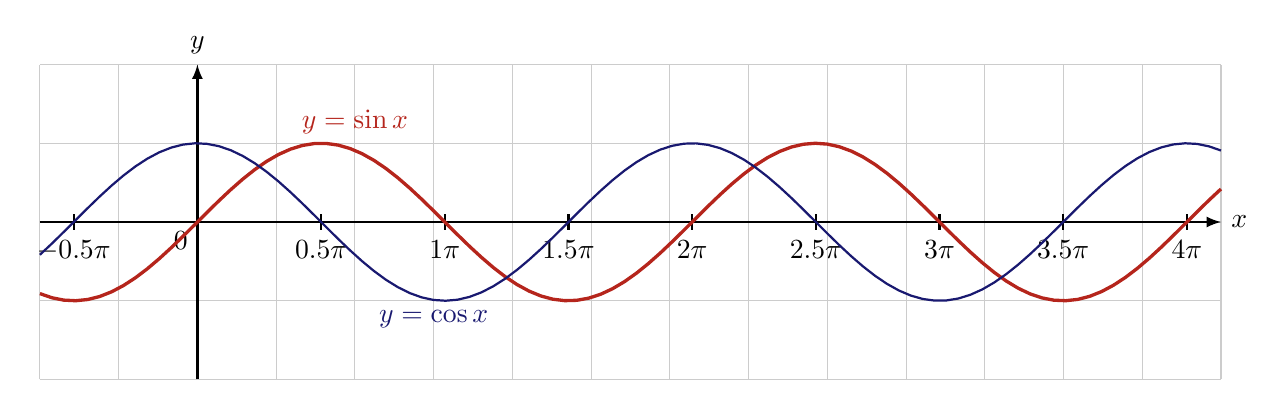
\begin{tikzpicture}
        \draw[thin,gray!40] (-2,-2) grid (13, 2);
        \draw[thick, ->, >=latex] (-2,0)--(13,0) node[right]{\(x\)};
        \draw[thick, ->, >=latex] (0,-2)--(0,2) node[above]{\(y\)};
        \draw (0, 0) node[below left] {0};

        \foreach \x in {-0.5, 0.5, 1, ..., 4} {
            \draw[thick] (\x*3.14159, 0.1) -- (\x*3.14159, -0.1) node[below] {\(\x\pi\)};
        }

        % \x r means to convert '\x' from degrees to radians:
        \draw [BrickRed, very thick, domain=-2:13, samples=100] plot (\x,{sin(\x r)});

        \draw [MidnightBlue, thick, domain=-2:13, samples=100] plot (\x,{cos(\x r)});

        \draw node[BrickRed, above] at (2, 1) {\(y = \sin{x}\)};
        \draw node[MidnightBlue, below] at (3, -1) {\(y = \cos{x}\)};
    \end{tikzpicture}
    
    \caption{The graph of the functions \(\sin{x}\) and \(\cos{x}\).}
    \label{fig:Ch02-trig-funcs-graph}
\end{figure}





\subsection{Exponential and logarithm}

One way to define the exponential function \(\exp\) is as follows.
%
\begin{align*}
    \exp(x + y) &= \exp(x) \cdot \exp(y)\\
    \exp(0) &= 1\\
    \frac{d}{dx} \exp(x) &= \exp(x) 
\end{align*}
%
Note that the first two relationships can be satisfied by any function of the form \(f(x) = a^x\) where \(a \in \mathbb{R}\). However, if we take all three conditions into account, the only function satisfying them is \(\exp(x) = e^x\), where \(e = 2.71828\cdots\) is Euler's number.

The exponential function \(\exp(x) = e^x\) is plotted in figure \ref{fig:Ch02-exp-graph}. Note that:
%
\begin{itemize}
    \item For all values of \(x\), we have \(\exp(x) > 0\).
    \item When \(x\) is negative, \(\exp(x)\) is very small.
    \item The value of \(\exp(x)\) grows very fast as \(x\) increases.
\end{itemize}

\begin{figure}[H]
    \centering

    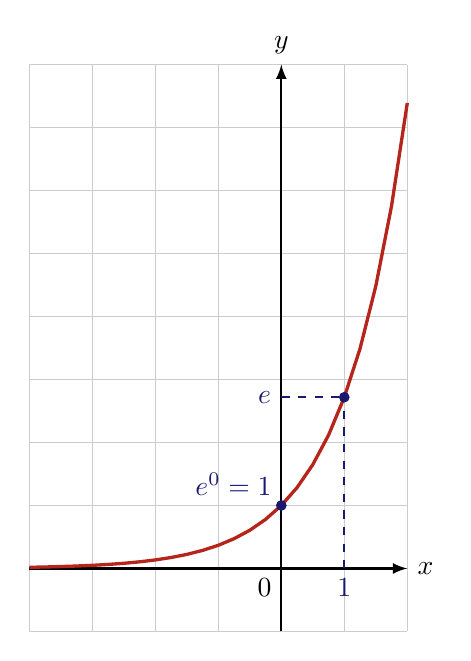
\begin{tikzpicture}[scale=0.8]
        \draw[thin,gray!40] (-4,-1) grid (2, 8);
        \draw[thick, ->, >=latex] (-4,0)--(2,0) node[right]{\(x\)};
        \draw[thick, ->, >=latex] (0,-1)--(0,8) node[above]{\(y\)};
        \draw (0, 0) node[below left] {0};

        \draw [BrickRed, very thick, domain=-4:2] plot (\x, {2.71828^\x}); 
        \filldraw[radius=0.075, MidnightBlue] (0,1) circle node[above left] {\(e^0 = 1\)};

        \draw[MidnightBlue, dashed, thick] (1, 0) node[below]{\(1\)} --(1, 2.71828);
        \draw[MidnightBlue, dashed, thick] (0, 2.71828) node[left]{\(e\)} --(1, 2.71828);

        \filldraw[radius=0.075, MidnightBlue] (1, 2.71828) circle;
    \end{tikzpicture}
    
    \caption{The graph of the function \(y = \exp(x) = e^x\).}
    \label{fig:Ch02-exp-graph}
\end{figure}

The natural logarithm \(\ln{x}\) is the inverse of the exponential, meaning that \(\ln(e^x) = x\). This results in the following properties.
%
\begin{align*}
    \ln(ab) &= \ln{a} + \ln{b}\\
    \ln\left(\frac{a}{b}\right) &= \ln{a} - \ln{b}\\
    \ln{1} &= 0\\
    \ln{e} &= 1\\
    a^x &= e^{x\ln{a}}\\
    \ln(a^x) &= x\ln{a}
\end{align*}
%
Since \(e^x > 0\) for all \(x\), the natural logarithm \(\ln{x}\) is only defined for positive values of \(x\).

The plot of \(y = \ln{x}\) is given in figure \ref{fig:Ch02-ln-graph}. Note that:
%
\begin{itemize}
    \item For \(x < 1\), we have \(\ln{x} < 0\).
    \item The curve intersects the \(x\)-axis at \((1, 0)\).
    \item For \(x > 1\), the value of \(\ln{x}\) grows very slowly as \(x\) increases.
\end{itemize}

\begin{figure}[H]
    \centering

    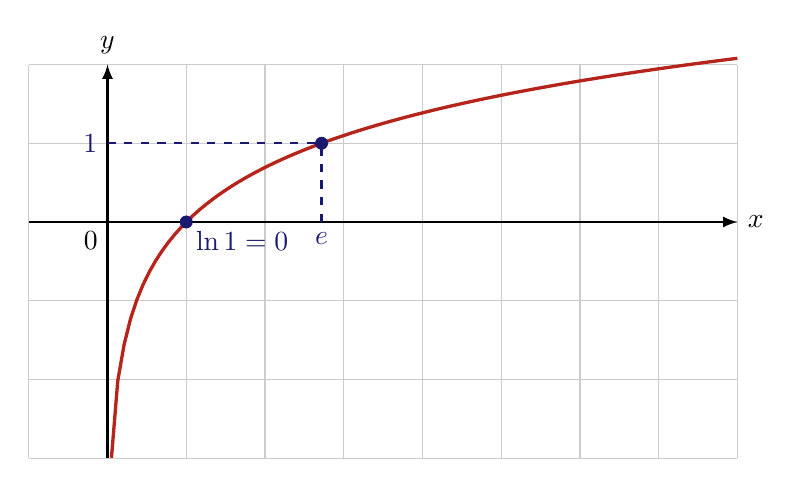
\begin{tikzpicture}
        \draw[thin,gray!40] (-1,-3) grid (8, 2);
        \draw[thick, ->, >=latex] (-1,0)--(8,0) node[right]{\(x\)};
        \draw[thick, ->, >=latex] (0,-3)--(0,2) node[above]{\(y\)};
        \draw (0, 0) node[below left] {0};

        \draw [BrickRed, very thick, domain=0.05:8, samples=100] plot (\x, {ln(\x)}); 
        \filldraw[radius=0.075, MidnightBlue] (1, 0) circle node[below right] {\(\ln{1} = 0\)};

        \draw[MidnightBlue, dashed, thick] (0, 1) node[left]{\(1\)} --(2.71828, 1);
        \draw[MidnightBlue, dashed, thick] (2.71828, 0) node[below]{\(e\)} --(2.71828, 1);

        \filldraw[radius=0.075, MidnightBlue] (2.71828, 1) circle;
    \end{tikzpicture}
    
    \caption{The graph of the function \(y = \exp(x) = e^x\).}
    \label{fig:Ch02-ln-graph}
\end{figure}




\subsection{Introduction to limits}

The idea of limits is simple.

\begin{quote}
    As \(x\) approaches a value, \(f(x)\) also approaches a value --- both possibly infinite. To denote this we write \(f(x) \rightarrow b\) as \(x \rightarrow a\), or \(\lim_{x \rightarrow a} f(x) = b\).
\end{quote}

This gives us four different cases.
%
\begin{itemize}
    \item As \(x\) approaches infinity, \(f(x)\) also approaches infinity. This means that \(f(x)\) can become arbitrarily large for large enough \(x\), i.e.
    %
    \[\forall d > 0,\; \exists c > 0,\; x > c \Rightarrow f(x) > d\text{.}\]
    %
    See figure \ref{fig:Ch02-lim-inf-inf}. (Restricting \(c\) and \(d\) to positive values is not strictly necessary, but it does make our lives easier in some cases.)

    \item As \(x\) approaches a value \(a\), \(f(x)\) approaches infinity. This means that \(f(x)\) can become arbitrarily large for \(x\) close enough \(x\), i.e.
    %
    \[\forall d > 0,\; \exists \eta > 0,\; 0 < \abs{x - a} < \eta \Rightarrow f(x) > d\text{.}\]
    %
    In other words, for any value \(d\), \(f(x)\) can be greater than \(d\) as long as the distance between \(x\) and \(a\) is less than some value \(\eta\). See figure \ref{fig:Ch02-lim-val-inf}.

    \item As \(x\) approaches infinity, \(f(x)\) approaches a value \(b\). This means that \(f(x)\) can get arbitrarily close to \(b\) for large enough \(x\), i.e.
    %
    \[\forall \epsilon > 0,\; \exists c > 0,\; x > c \Rightarrow \abs{f(x) - b} < \epsilon\text{.}\]
    %
    See figure \ref{fig:Ch02-lim-inf-val}.
    
    \item As \(x\) approaches a value \(a\), \(f(x)\) approaches a value \(b\). This means that \(f(x)\) can become arbitrarily close to \(b\) for \(x\) close enough to \(a\), i.e.
    %
    \[\forall \epsilon > 0,\; \exists \eta > 0,\; 0 < \abs{x - a} < \eta \Rightarrow \abs{f(x) - b} < \epsilon\text{.}\]
    %
    See figure \ref{fig:Ch02-lim-val-val}.
\end{itemize}

\begin{figure}[H]
    \centering

    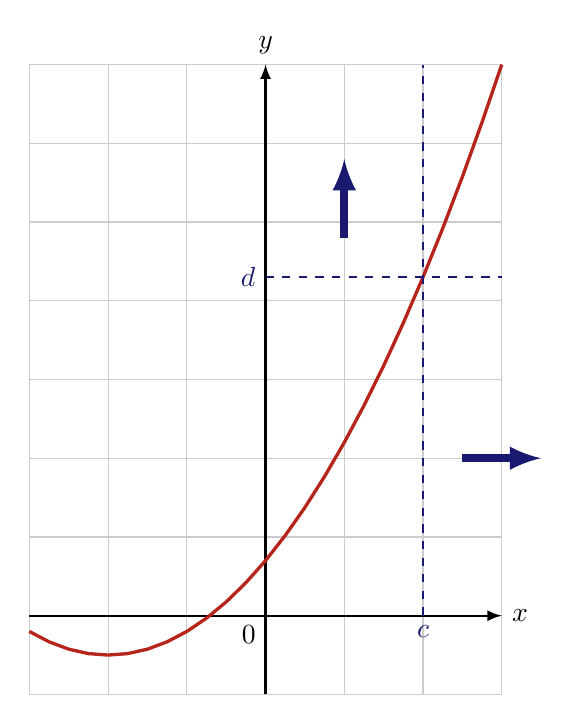
\begin{tikzpicture}
        \draw[thin,gray!40] (-3,-1) grid (3, 7);
        \draw[thick, ->, >=latex] (-3,0)--(3,0) node[right]{\(x\)};
        \draw[thick, ->, >=latex] (0,-1)--(0,7) node[above]{\(y\)};
        \draw (0, 0) node[below left] {0};

        \draw [BrickRed, very thick, domain=-3:3] plot (\x, {0.3*(\x + 2)^2 - 0.5}); 

        \draw[MidnightBlue, dashed, thick] (2, 0) node[below]{\(c\)} --(2, 7);
        \draw[MidnightBlue, dashed, thick] (0, 4.3) node[left]{\(d\)} -- (3, 4.3);

        \draw[MidnightBlue, line width=1mm, -latex] (1, 4.8) -- (1, 5.8);

        \draw[MidnightBlue, line width=1mm, -latex] (2.5, 2) -- (3.5, 2);
    \end{tikzpicture}
    
    \caption{As \(x\) approaches infinity, so does \(f(x)\).}
    \label{fig:Ch02-lim-inf-inf}
\end{figure}

\begin{figure}[H]
    \centering

    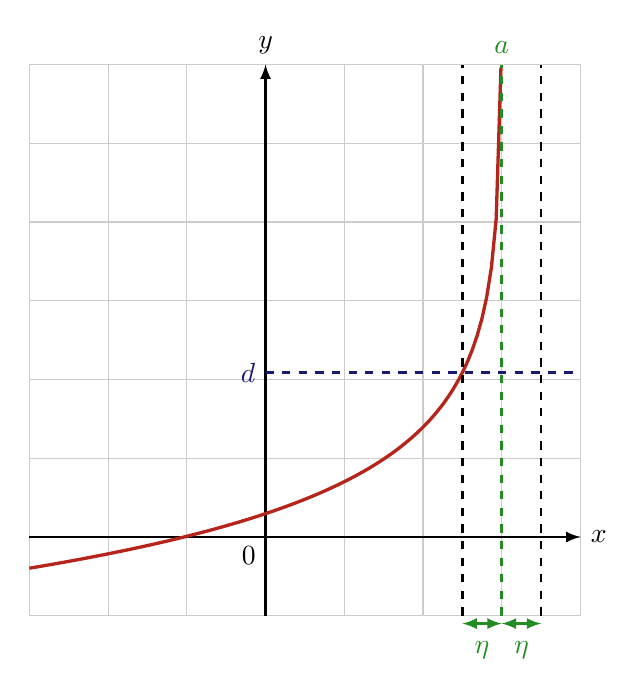
\begin{tikzpicture}
        \draw[thin,gray!40] (-3,-1) grid (4, 6);
        \draw[thick, ->, >=latex] (-3,0)--(4,0) node[right]{\(x\)};
        \draw[thick, ->, >=latex] (0,-1)--(0,6) node[above]{\(y\)};
        \draw (0, 0) node[below left] {0};

        \draw [BrickRed, very thick, domain=-3:2.99, samples=100] plot (\x, {6-ln(300-100*\x)}); 

        \draw[dashed, thick] (2.5, -1) -- (2.5, 6);
        \draw[dashed, thick] (3.5, -1) -- (3.5, 6);
        \draw[MidnightBlue, dashed, thick] (0, 2.09) node[left]{\(d\)} -- (4, 2.09);

        \draw[ForestGreen, very thick, dashed] (3, -1) -- (3, 6) node[above]{\(a\)};

        \draw[ForestGreen, thick, latex-latex, shift={(0, -0.1)}] (2.5, -1) -- (3, -1) node[pos=0.5, below, shift={(0, -0.1)}] {\(\eta\)};

        \draw[ForestGreen, thick, latex-latex, shift={(0, -0.1)}] (3, -1) -- (3.5, -1) node[pos=0.5, below, shift={(0, -0.1)}] {\(\eta\)};
    \end{tikzpicture}
    
    \caption{As \(x\) approaches \(a\), \(f(x)\) approaches infinity.}
    \label{fig:Ch02-lim-val-inf}
\end{figure}

\begin{figure}[H]
    \centering

    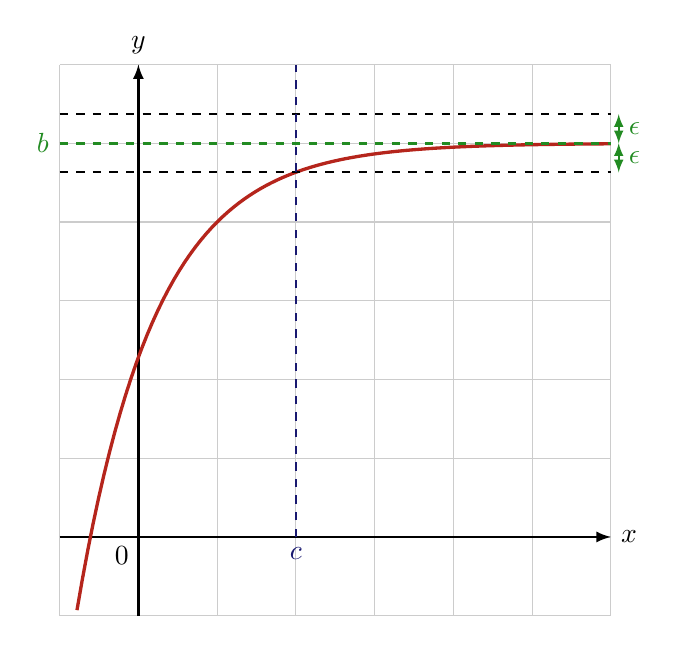
\begin{tikzpicture}
        \draw[thin,gray!40] (-1,-1) grid (6, 6);
        \draw[thick, ->, >=latex] (-1,0)--(6,0) node[right]{\(x\)};
        \draw[thick, ->, >=latex] (0,-1)--(0,6) node[above]{\(y\)};
        \draw (0, 0) node[below left] {0};

        \draw [BrickRed, very thick, domain=-0.78:6, samples=100] plot (\x, {5-2.71828^(1-\x)}); 

        \draw[dashed, thick] (-1, 4.63) -- (6, 4.63);
        \draw[dashed, thick] (-1, 5.37) -- (6, 5.37);
        \draw[MidnightBlue, dashed, thick] (2, 0) node[below]{\(c\)} -- (2, 6);

        \draw[ForestGreen, very thick, dashed] (-1, 5) node[left]{\(b\)}-- (6, 5);

        \draw[ForestGreen, semithick, latex-latex, shift={(0.1, 0)}] (6, 5.37) -- (6, 5) node[pos=0.5, right] {\(\epsilon\)};

        \draw[ForestGreen, semithick, latex-latex, shift={(0.1, 0)}] (6, 5) -- (6, 4.63) node[pos=0.5, right] {\(\epsilon\)};
    \end{tikzpicture}
    
    \caption{As \(x\) approaches infinity, \(f(x)\) approaches \(b\).}
    \label{fig:Ch02-lim-inf-val}
\end{figure}

\begin{figure}[H]
    \centering

    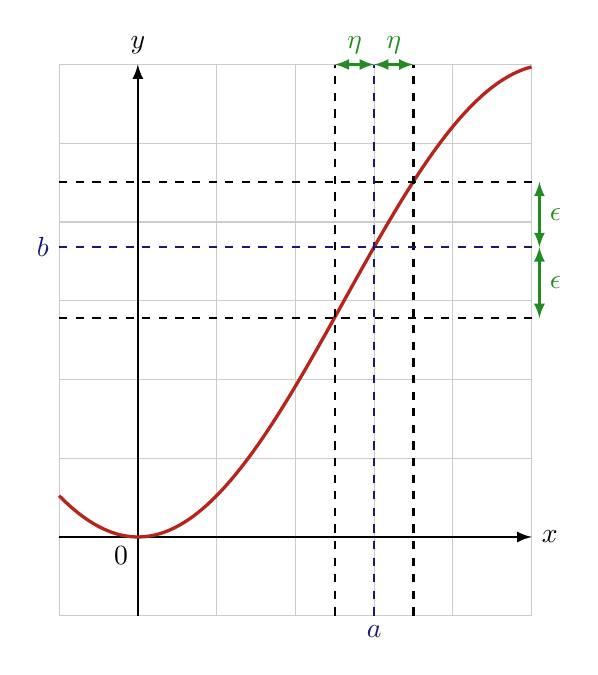
\begin{tikzpicture}
        \draw[thin,gray!40] (-1,-1) grid (5, 6);
        \draw[thick, ->, >=latex] (-1,0)--(5,0) node[right]{\(x\)};
        \draw[thick, ->, >=latex] (0,-1)--(0,6) node[above]{\(y\)};
        \draw (0, 0) node[below left] {0};

        \draw [BrickRed, very thick, domain=-1:5, samples=100] plot (\x, {6*(sin((0.3*\x) r))^2}); 

        \draw[dashed, thick] (-1, 2.78) -- (5, 2.78);
        \draw[dashed, thick] (-1, 4.51) -- (5, 4.51);

        \draw[dashed, thick] (2.5, -1) -- (2.5, 6);
        \draw[dashed, thick] (3.5, -1) -- (3.5, 6);

        \draw[MidnightBlue, dashed, thick] (3, -1) node[below]{\(a\)} -- (3, 6);
        \draw[MidnightBlue, dashed, thick] (-1, 3.68) node[left]{\(b\)} -- (5, 3.68);

        \draw[ForestGreen, thick, latex-latex] (2.5, 6) -- (3, 6) node[pos=0.5, above] {\(\eta\)};

        \draw[ForestGreen, thick, latex-latex] (3, 6) -- (3.5, 6) node[pos=0.5, above] {\(\eta\)};

        \draw[ForestGreen, thick, latex-latex, shift={(0.1, 0)}] (5, 2.78) -- (5, 3.68) node[pos=0.5, right] {\(\epsilon\)};

        \draw[ForestGreen, thick, latex-latex, shift={(0.1, 0)}] (5, 3.68) -- (5, 4.51) node[pos=0.5, right] {\(\epsilon\)};
    \end{tikzpicture}
    
    \caption{As \(x\) approaches \(a\), \(f(x)\) approaches \(b\).}
    \label{fig:Ch02-lim-val-val}
\end{figure}

A limit that exists is known as a \textit{finite} limit. Finite limits can be combined in a natural way.
%
\begin{align*}
    \lim_{x \rightarrow a} (f(x) + g(x)) &= \lim_{x \rightarrow a} f(x) + \lim_{x \rightarrow a} g(x)\\
    \lim_{x \rightarrow a} (f(x) \cdot g(x)) &= \lim_{x \rightarrow a} f(x) \cdot \lim_{x \rightarrow a} g(x)\\
    \lim_{x \rightarrow a} \frac{f(x)}{g(x)} &= \frac{\lim_{x \rightarrow a} f(x)}{\lim_{x \rightarrow a} g(x)}
\end{align*}

We use the following rules to handle infinities.
%
\begin{align*}
    a \times \infty &= \infty\\
    \frac{a}{\infty} &= 0
\end{align*}

If a limit involves \(x\) approaching zero, we may sometimes have to specify the direction in which \(x\) is approaching it, i.e. whether it is approaching zero as a positive number (from the right) or as a negative number (from the left).
%
\begin{align*}
    \lim_{x \rightarrow 0^+} \frac{1}{x} &= \infty\\
    \lim_{x \rightarrow 0^-} \frac{1}{x} &= -\infty
\end{align*}

There are certain cases where we \textit{cannot} combine limits. These are called \textit{indeterminate forms}, and there is no general rule for figuring out what these indeterminate forms evaluate to. Examples of indeterminate forms are given below.
%
\[
\frac{0}{0},\; \frac{\infty}{\infty},\; 0 \times \infty,\; \infty - \infty,\; 0^0,\; 1^\infty,\; \infty^0
\]




\subsection{Little o and big O notation}

Here we introduce two types of notation: little \(o\) and big \(O\).
%
\begin{quote}
    \textbf{Little \(\mathbf{o}\) notation.}

    We write \(f = o(g)\) near a value \(b\) if \(\lim_{x \rightarrow b} \frac{f(x)}{g(x)} = 0\). This means that \(f\) is negligible when compared with \(g\) (or that \(g\) is more significant than \(f\)) near \(b\).
    
    For example, we say that \(x = o(x^2)\) near \(\infty\) because \(\lim_{x\rightarrow \infty} x / x^2 = 0\).

    \vspace{1em}

    \textbf{Big \(\mathbf{O}\) notation.}

    We write \(f = O(g)\) near a value \(b\) if \(\lim_{x \rightarrow b} \left|\frac{f(x)}{g(x)}\right|\) is bounded. We can express the idea of being ``bounded'' more precisely as
    %
    \[\exists M \in \mathbb{R},\; \lim_{x \rightarrow b} \left|\frac{f(x)}{g(x)}\right| < M\text{.}\]
    %
    This means that \(f\) and \(g\) have a similar growth rate near \(b\).

    For example, we say that \(3x = O(x+1)\) near \(\infty\) because \(\lim_{x \rightarrow \infty} \left|\frac{3x}{x+1}\right| < \frac{3x}{x} = 3\).
\end{quote}
%
Notice that by definition, we have \(f = o(g) \;\Rightarrow\; f = O(g)\). This is because if \(f = o(g)\) is true, then the limit \(\lim_{x \rightarrow b} \frac{f(x)}{g(x)}\) must equal zero and is therefore bounded, which gives us \(f = O(g)\).






\subsection{Continuity}

A function \(f\) is continuous if for all \(a\) where \(f(a)\) is defined, we have \(\lim_{x\rightarrow a} f(x) = f(a)\).

In practice, this means that the graph of \(y = f(x)\) is a single unbroken curve. The exponential and logarithm functions, for example, are both continuous.

An important result of this is the \textit{intermediate value theorem}.
%
\begin{quote}
    \textbf{Intermediate value theorem.}

    Assume for a continuous function \(f\) that \(a < b\) and \(f(a) < f(b)\). For any value \(y\) such that \(f(a) < y < f(b)\), there exists a (not necessarily unique) value \(x\) such that \(a < x < b\) and \(f(x) = y\).
\end{quote}
%
See figure \ref{fig:Ch02-int-value-thm} and \ref{fig:Ch02-int-value-thm-uniqueness}.

\begin{figure}[H]
    \centering

    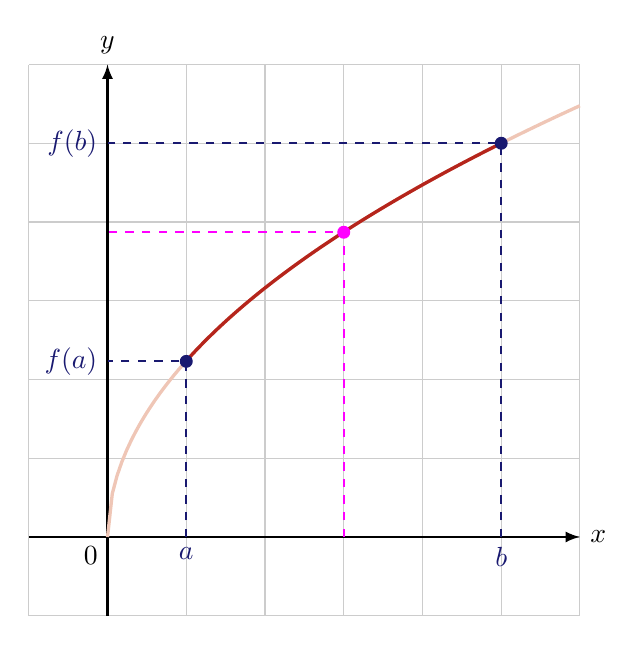
\begin{tikzpicture}
        \draw[thin,gray!40] (-1,-1) grid (6, 6);
        \draw[thick, ->, >=latex] (-1,0)--(6,0) node[right]{\(x\)};
        \draw[thick, ->, >=latex] (0,-1)--(0,6) node[above]{\(y\)};
        \draw (0, 0) node[below left] {0};

        \draw [BrickRed!20, very thick, domain=0:6, samples=100] plot (\x,
        {sqrt(5*\x)});

        \draw [BrickRed, very thick, domain=1:5, samples=100] plot (\x,
        {sqrt(5*\x)});

        \filldraw[radius=0.075, MidnightBlue] (1, 2.23) circle;
        \draw[dashed, MidnightBlue, thick] (1, 0) node[below]{\(a\)} -- (1, 2.23) -- (0, 2.23) node[left]{\(f(a)\)};

        \filldraw[radius=0.075, Fuchsia] (3, 3.87) circle;
        \draw[dashed, Fuchsia, thick] (3, 0) -- (3, 3.87) -- (0, 3.87);


        \filldraw[radius=0.075, MidnightBlue] (5, 5) circle;
        \draw[dashed, MidnightBlue, thick] (5, 0) node[below]{\(b\)} -- (5, 5) -- (0, 5) node[left]{\(f(b)\)};
    \end{tikzpicture}
    
    \caption{The intermediate value theorem.}
    \label{fig:Ch02-int-value-thm}
\end{figure}


\begin{figure}[H]
    \centering

    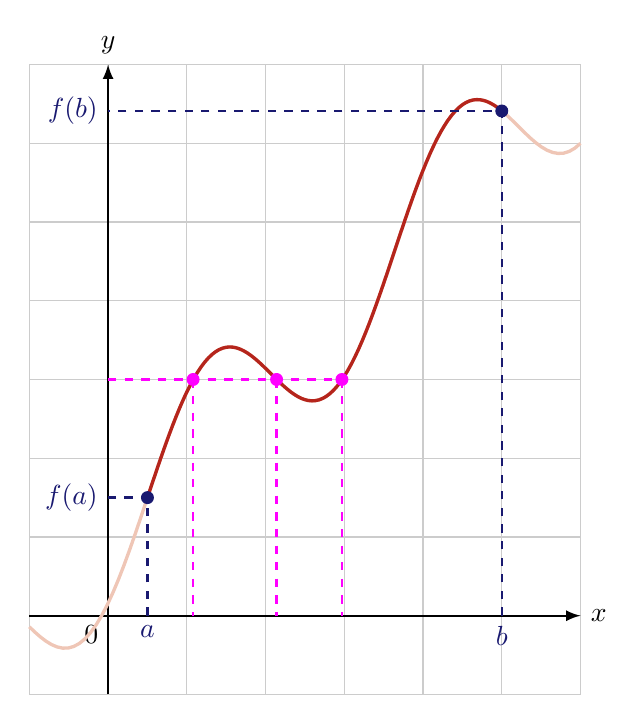
\begin{tikzpicture}
        \draw[thin,gray!40] (-1,-1) grid (6, 7);
        \draw[thick, ->, >=latex] (-1,0)--(6,0) node[right]{\(x\)};
        \draw[thick, ->, >=latex] (0,-1)--(0,7) node[above]{\(y\)};
        \draw (0, 0) node[below left] {0};

        \draw [BrickRed!20, very thick, domain=-1:6, samples=100] plot (\x,
        {sin((2*\x-1) r)+\x+1});

        \draw [BrickRed, very thick, domain=0.5:5, samples=100] plot (\x,
        {sin((2*\x-1) r)+\x+1});

        \filldraw[radius=0.075, MidnightBlue] (0.5, 1.5) circle;
        \draw[dashed, MidnightBlue, thick] (0.5, 0) node[below]{\(a\)} -- (0.5, 1.5) -- (0, 1.5) node[left]{\(f(a)\)};

        \filldraw[radius=0.075, Fuchsia] (1.08, 3) circle;
        \draw[dashed, Fuchsia, thick] (1.08, 3) -- (1.08, 0);
        \filldraw[radius=0.075, Fuchsia] (2.14, 3) circle;
        \draw[dashed, Fuchsia, thick] (2.14, 3) -- (2.14, 0);
        \filldraw[radius=0.075, Fuchsia] (2.97, 3) circle;
        \draw[dashed, Fuchsia, thick] (2.97, 3) -- (2.97, 0);

        \draw[dashed, Fuchsia, thick] (0, 3) -- (2.97, 3);

        \filldraw[radius=0.075, MidnightBlue] (5, 6.41) circle;
        \draw[dashed, MidnightBlue, thick] (5, 0) node[below]{\(b\)} -- (5, 6.41) -- (0, 6.41) node[left]{\(f(b)\)};
    \end{tikzpicture}
    
    \caption{In the intermediate value theorem, for a given value \(y\), the value of \(x\) does not necessarily have to be unique.}
    \label{fig:Ch02-int-value-thm-uniqueness}
\end{figure}